\documentclass[11pt]{article}
\usepackage{amsmath}
\usepackage{amssymb}
\usepackage{graphicx}
\usepackage{tabularx}
\usepackage{fancyhdr}
\usepackage{lastpage}

% Page layout
\usepackage[top=1in, bottom=1in, left=1in, right=1in]{geometry}

% Header and footer
\pagestyle{fancy}
\fancyhf{}
\rfoot{Page \thepage}
\renewcommand{\headrulewidth}{0pt}

% Modified Question command with left-aligned number
\newcommand{\questiona}[2]{
    \noindent\textbf{Q#2.} #1 \hfill \textbf{[1 Mark]}
}

\newcommand{\questionb}[2]{
    \noindent\textbf{Q#2.} #1 \hfill \textbf{[2 Marks]}
}

\begin{document}

% Title section with horizontal line
\begin{center}
    \Large\textbf{GATE 2018 - Architecture and Planning (AR)} \\
    \large\textbf{General Aptitude and Technical Questions} \\
    \rule{\textwidth}{0.5pt} % Horizontal line below heading
\end{center}

\vspace{0.5cm}

% General Aptitude Section
\section*{General Aptitude}

\questiona{"When she fell down the \_\_\_\_\_, she received many \_\_\_\_\_ but little help." The words that best fill the blanks in the above sentence are}{1}
\begin{enumerate}
    \item[(A)] stairs, stares  
    \item[(B)] stairs, stairs  
    \item[(C)] stares, stairs  
    \item[(D)] stares, stares  
\end{enumerate}
\vspace{0.5cm}

\questiona{"In spite of being warned repeatedly, he failed to correct his \_\_\_\_\_ behaviour." The word that best fills the blank in the above sentence is}{2}
\begin{enumerate}
    \item[(A)] rational  
    \item[(B)] reasonable  
    \item[(C)] errant  
    \item[(D)] good  
\end{enumerate}
\vspace{0.5cm}

\questiona{For \(0 \leq x \leq 2\pi\), \(\sin x\) and \(\cos x\) are both decreasing functions in the interval \_\_\_\_\_.}{3}
\begin{enumerate}
    \item[(A)] \(\left(0, \frac{\pi}{2}\right)\)  
    \item[(B)] \(\left(\frac{\pi}{2}, \pi\right)\)  
    \item[(C)] \(\left(\pi, \frac{3\pi}{2}\right)\)  
    \item[(D)] \(\left(\frac{3\pi}{2}, 2\pi\right)\)  
\end{enumerate}
\vspace{0.5cm}

\questiona{The area of an equilateral triangle is \(\sqrt{3}\). What is the perimeter of the triangle?}{4}
\begin{enumerate}
    \item[(A)] 2  
    \item[(B)] 4  
    \item[(C)] 6  
    \item[(D)] 8  
\end{enumerate}
\vspace{0.5cm}

\questiona{Arrange the following three-dimensional objects in the descending order of their volumes:
\begin{enumerate}
    \item A cuboid with dimensions 10 cm, 8 cm and 6 cm
    \item A cube of side 8 cm
    \item A cylinder with base radius 7 cm and height 7 cm
    \item A sphere of radius 7 cm
\end{enumerate}}{5}
\begin{enumerate}
    \item[(A)] (i), (ii), (iii), (iv)  
    \item[(B)] (ii), (i), (iv), (iii)  
    \item[(C)] (iii), (ii), (i), (iv)  
    \item[(D)] (iv), (iii), (ii), (i)  
\end{enumerate}
\vspace{0.5cm}

\questionb{An automobile travels from city A to city B and returns to city A by the same route. The speed of the vehicle during the onward and return journeys were constant at 60 km/h and 90 km/h, respectively. What is the average speed in km/h for the entire journey?}{6}
\begin{enumerate}
    \item[(A)] 72  
    \item[(B)] 73  
    \item[(C)] 74  
    \item[(D)] 75  
\end{enumerate}
\vspace{0.5cm}

\questionb{A set of 4 parallel lines intersect with another set of 5 parallel lines. How many parallelograms are formed?}{7}
\begin{enumerate}
    \item[(A)] 20  
    \item[(B)] 48  
    \item[(C)] 60  
    \item[(D)] 72  
\end{enumerate}
\vspace{0.5cm}

\questionb{To pass a test, a candidate needs to answer at least 2 out of 3 questions correctly. A total of 6,30,000 candidates appeared for the test. Question A was correctly answered by 3,30,000 candidates. Question B was answered correctly by 2,50,000 candidates. Question C was answered correctly by 2,60,000 candidates. Both questions A and B were answered correctly by 1,00,000 candidates. Both questions B and C were answered correctly by 90,000 candidates. Both questions A and C were answered correctly by 80,000 candidates. If the number of students answering all questions correctly is the same as the number answering none, how many candidates failed to clear the test?}{8}
\begin{enumerate}
    \item[(A)] 30,000  
    \item[(B)] 2,70,000  
    \item[(C)] 3,90,000  
    \item[(D)] 4,20,000  
\end{enumerate}
\vspace{0.5cm}

\questionb{If \(x^2 + x - 1 = 0\) what is the value of \(x^4 + \frac{1}{x^4}\)?}{9}
\begin{enumerate}
    \item[(A)] 1  
    \item[(B)] 5  
    \item[(C)] 7  
    \item[(D)] 9  
\end{enumerate}
\vspace{0.5cm}

\questionb{In a detailed study of annual crow births in India, it was found that there was relatively no growth during the period 2002 to 2004 and a sudden spike from 2004 to 2005. In another unrelated study, it was found that the revenue from cracker sales in India which remained fairly flat from 2002 to 2004, saw a sudden spike in 2005 before declining again in 2006. The solid line in the graph below refers to annual sale of crackers and the dashed line refers to the annual crow births in India. Choose the most appropriate inference from the above data.}{10}
\begin{center}
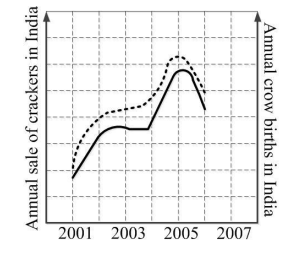
\includegraphics[width=0.5\textwidth]{figures/10.png}
\end{center}
\begin{enumerate}
    \item[(A)] There is a strong correlation between crow birth and cracker sales.  
    \item[(B)] Cracker usage increases crow birth rate.  
    \item[(C)] If cracker sale declines, crow birth will decline.  
    \item[(D)] Increased birth rate of crows will cause an increase in the sale of crackers.  
\end{enumerate}
\vspace{0.5cm}

% Technical Section
\section*{Technical Section}

\questiona{In a Colour Wheel, Red and Blue colours are}{1}
\begin{enumerate}
    \item[(A)] Tertiary  
    \item[(B)] Complementary  
    \item[(C)] Secondary  
    \item[(D)] Primary  
\end{enumerate}
\vspace{0.5cm}

\questiona{In a bird's eye perspective view of a cuboid, the maximum number of vanishing points is}{2}
\begin{enumerate}
    \item[(A)] 1  
    \item[(B)] 2  
    \item[(C)] 3  
    \item[(D)] 6  
\end{enumerate}
\vspace{0.5cm}

\questiona{The compressive strength of M-25 concrete is}{3}
\begin{enumerate}
    \item[(A)] 25 kg/sqm  
    \item[(B)] 25 N/sqmm  
    \item[(C)] 250 N/sqmm  
    \item[(D)] 2.5 N/sqmm  
\end{enumerate}
\vspace{0.5cm}

\questiona{In Critical Path Method (CPM) for time scheduling, 'forward pass calculation' is carried out for determining}{4}
\begin{enumerate}
    \item[(A)] Late start and early finish time  
    \item[(B)] Early start and early finish time  
    \item[(C)] Late start and late finish time  
    \item[(D)] Early start and late finish time  
\end{enumerate}
\vspace{0.5cm}

\questiona{Collapse of the World Trade Center (WTC), New York, in 2001, was due to}{5}
\begin{enumerate}
    \item[(A)] Wind load failure  
    \item[(B)] Foundation failure  
    \item[(C)] Thermal performance failure of reinforcement steel in RCC  
    \item[(D)] Thermal performance failure of structural steel  
\end{enumerate}
\vspace{0.5cm}

\questiona{During the construction of tall buildings, the equipment used for hoisting building materials to the upper floors is a}{6}
\begin{enumerate}
    \item[(A)] Goods lift  
    \item[(B)] Capsule lift  
    \item[(C)] Gantry crane  
    \item[(D)] Tower crane  
\end{enumerate}
\vspace{0.5cm}

\questiona{A Rock-cut style of architecture is represented by}{7}
\begin{enumerate}
    \item[(A)] Shyama Rama Temple, Bishnupur  
    \item[(B)] Kailasa Temple, Ellora  
    \item[(C)] Kandariya Mahadeva Temple, Khajuraho  
    \item[(D)] Sanchi Stupa, Sanchi  
\end{enumerate}
\vspace{0.5cm}

\questiona{'Area based development' and 'Pan city development' are part of}{8}
\begin{enumerate}
    \item[(A)] Smart City Mission  
    \item[(B)] Digital India Mission  
    \item[(C)] Swachh Bharat Mission  
    \item[(D)] Atal Innovation Mission  
\end{enumerate}
\vspace{0.5cm}

\questiona{In mass transportation, LRTS stands for}{9}
\begin{enumerate}
    \item[(A)] Light Rail Transit System  
    \item[(B)] Linear Rail Transit System  
    \item[(C)] Light Rail Transportation System  
    \item[(D)] Linear Rail Transportation System  
\end{enumerate}
\vspace{0.5cm}

\questiona{The structural grid type shown in the figure below is a}{10}
\begin{center}
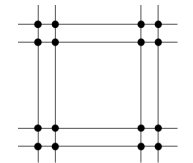
\includegraphics[width=0.5\textwidth]{figures/10a.png}
\end{center}
\begin{enumerate}
    \item[(A)] Tartan Grid  
    \item[(B)] Square Grid  
    \item[(C)] Rectangular Grid  
    \item[(D)] Irregular Grid  
\end{enumerate}
\vspace{0.5cm}

\questiona{Assuming other variables remaining constant, the Tropical Summer Index}{11}
\begin{enumerate}
    \item[(A)] Increases with increase in air velocity  
    \item[(B)] Decreases with increase in wet-bulb temperature  
    \item[(C)] Decreases with increase in globe temperature  
    \item[(D)] Increases with increase in vapour pressure  
\end{enumerate}
\vspace{0.5cm}

\questiona{Government of India's urban development program 'HRIDAY' stands for}{12}
\begin{enumerate}
    \item[(A)] Heritage Rejuvenation Implementation Development Aayog Yojana  
    \item[(B)] Heritage Review Implementation Development Augmentation Yojana  
    \item[(C)] Heritage City Development and Augmentation Yojana  
    \item[(D)] Heritage City Improvement and Development Aawas Yojana  
\end{enumerate}
\vspace{0.5cm}

\questiona{As per the Urban and Regional Development Plan Formulation and Implementation (URDPFI) guidelines, the plan period considered in a 'Perspective plan' is}{13}
\begin{enumerate}
    \item[(A)] 1-10 years  
    \item[(B)] 11-15 years  
    \item[(C)] 20-30 years  
    \item[(D)] 35-45 years  
\end{enumerate}
\vspace{0.5cm}

\questiona{The Hall of Nations, New Delhi, was designed by}{14}
\begin{enumerate}
    \item[(A)] Charles Correa  
    \item[(B)] Raj Rewal  
    \item[(C)] Joseph Allen Stein  
    \item[(D)] A. P. Kanyinde  
\end{enumerate}
\vspace{0.5cm}

\questiona{As per the National Building Code of India 2016, the minimum turning radius (in metres) required for fire tender movement is}{15}
\begin{enumerate}
    \item[(A)] 8.0  
    \item[(B)] 8.5  
    \item[(C)] 9.0  
    \item[(D)] 9.5  
\end{enumerate}
\vspace{0.5cm}

\questiona{Sidi Bashir Mosque with 'Shaking Minarets' is located in}{16}
\begin{enumerate}
    \item[(A)] Ajmer  
    \item[(B)] Allahabad  
    \item[(C)] Ahmedabad  
    \item[(D)] Amritsar  
\end{enumerate}
\vspace{0.5cm}

\questiona{'Sight Distance' is considered in the design of}{17}
\begin{enumerate}
    \item[(A)] Road intersection  
    \item[(B)] Fenestration  
    \item[(C)] Open kitchen  
    \item[(D)] Auditorium  
\end{enumerate}
\vspace{0.5cm}

\questiona{In India, the term 'Town Planning Scheme' refers to}{18}
\begin{enumerate}
    \item[(A)] Land renewal  
    \item[(B)] Land rejuvenation  
    \item[(C)] Land reclamation  
    \item[(D)] Land readjustment  
\end{enumerate}
\vspace{0.5cm}

\questiona{Bamboo is a type of}{19}
\begin{enumerate}
    \item[(A)] Shrub  
    \item[(B)] Timber  
    \item[(C)] Evergreen tree  
    \item[(D)] Perennial grass  
\end{enumerate}
\vspace{0.5cm}

\questiona{According to the UN, one of the components for measuring 'inclusive growth' is}{20}
\begin{enumerate}
    \item[(A)] Economic well-being  
    \item[(B)] Physical infrastructure  
    \item[(C)] Education  
    \item[(D)] Life expectancy  
\end{enumerate}
\vspace{0.5cm}

\questiona{The unit of measurement of Damp Proof Course (DPC) in building construction is}{21}
\begin{enumerate}
    \item[(A)] kg  
    \item[(B)] cum  
    \item[(C)] sqm  
    \item[(D)] rm  
\end{enumerate}
\vspace{0.5cm}

\questiona{Which of the following is NOT a Building Information Modeling software tool}{22}
\begin{enumerate}
    \item[(A)] Adobe Illustrator  
    \item[(B)] Bentley Microstation  
    \item[(C)] Autodesk Revit  
    \item[(D)] Graphisoft ARCHICAD  
\end{enumerate}
\vspace{0.5cm}

\questiona{The concentric circles in a solar chart represent}{23}
\begin{enumerate}
    \item[(A)] Azimuth angle  
    \item[(B)] Altitude angle  
    \item[(C)] Horizontal shadow angle  
    \item[(D)] Vertical shadow angle  
\end{enumerate}
\vspace{0.5cm}

\questiona{A room of 3m × 3m × 3m has a reverberation time of 0.8 sec. Using Sabine's method, the total absorption in the room is \_\_\_\_\_ sabin (up to one decimal place).}{24}
\vspace{0.5cm}

\questiona{A 25 storeyed building has 5 lifts. The resulting waiting time is 35 sec and 'Return Travel Time' is 175 sec. The number of lifts required for reducing waiting time to 25 sec, without increasing the lift speed, is \_\_\_\_\_.}{25}
\vspace{0.5cm}

\questionb{Match the planning documents in Group-I with their respective government schemes in Group-II}{26}
\begin{tabularx}{\textwidth}{|l|X|}
\hline
\textbf{Group-I} & \textbf{Group-II} \\
\hline
P Integrated Cluster Action Plan & 1 NULM \\
Q Service Level Improvement Plan & 2 Make in India \\
R Housing for All Plan of Action & 3 RuRBAN mission \\
S City Livelihood Centre Development Plan & 4 PMAY \\
 & 5 AMRUT \\
\hline
\end{tabularx}
\begin{enumerate}
    \item[(A)] P-4, Q-1, R-5, S-2
    \item[(B)] P-3, Q-5, R-4, S-2
    \item[(C)] P-5, Q-1, R-4, S-3
    \item[(D)] P-3, Q-5, R-4, S-1
\end{enumerate}
\vspace{0.5cm}

\questionb{Associate the fire safety requirements for high rise buildings in Group-I with corresponding standards of the National Building Code of India 2016 in Group-II}{27}
\begin{tabularx}{\textwidth}{|l|X|}
\hline
\textbf{Group-I} & \textbf{Group-II} \\
\hline
P Minimum Refuge area & 1 12.5 sqm/person \\
Q Maximum Travel distance & 2 2.0 m \\
R Maximum Occupant load & 3 0.3 sqm/person \\
S Minimum Stair case width & 4 12.0 ton \\
 & 5 30.0 m \\
\hline
\end{tabularx}
\begin{enumerate}
    \item[(A)] P-4, Q-1, R-5, S-2
    \item[(B)] P-3, Q-5, R-4, S-1
    \item[(C)] P-3, Q-5, R-1, S-2
    \item[(D)] P-4, Q-5, R-1, S-3
\end{enumerate}
\vspace{0.5cm}

\questionb{Match the photometric quantities in Group-I with their respective units in Group-II}{28}
\begin{tabularx}{\textwidth}{|l|X|}
\hline
\textbf{Group-I} & \textbf{Group-II} \\
\hline
P Illuminance & 1 Candela \\
Q Luminous Intensity & 2 Candela/sqm \\
R Luminance & 3 Lumens/sqm \\
S Luminous Efficacy & 4 Lumens/watt \\
 & 5 Lumens \\
\hline
\end{tabularx}
\begin{enumerate}
    \item[(A)] P-3, Q-2, R-5, S-4
    \item[(B)] P-5, Q-4, R-2, S-1
    \item[(C)] P-5, Q-1, R-2, S-3
    \item[(D)] P-3, Q-1, R-2, S-4
\end{enumerate}
\vspace{0.5cm}

\questionb{Associate the symbols in Group I with their meanings in Group II}{29}
\begin{center}
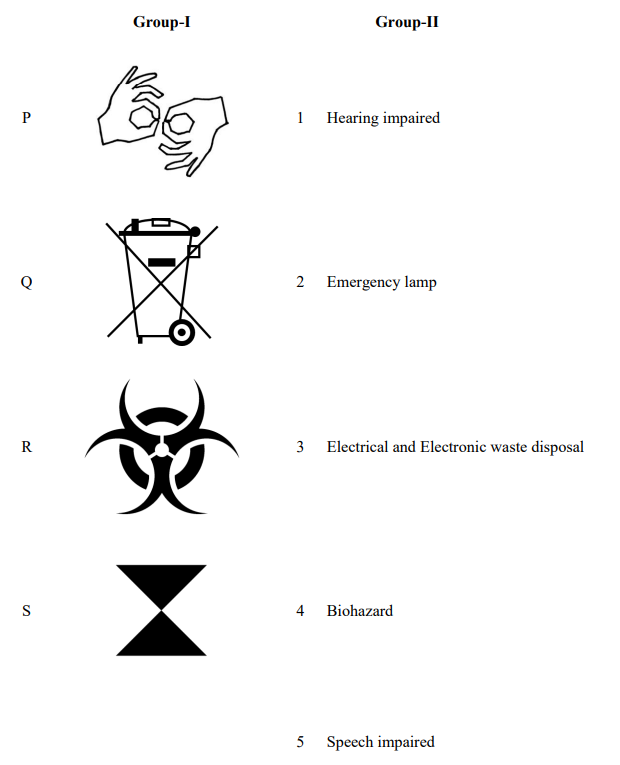
\includegraphics[width=0.8\textwidth]{figures/29.png}
\end{center}

\begin{enumerate}
    \item[(A)] P-5, Q-3, R-1, S-2
    \item[(B)] P-1, Q-5, R-3, S-4
    \item[(C)] P-1, Q-3, R-4, S-5
    \item[(D)] P-5, Q-3, R-4, S-2
\end{enumerate}
\vspace{0.5cm}

\questionb{Match the elements in Group-I with the building components in Group-II}{30}
\begin{tabularx}{\textwidth}{|l|X|}
\hline
\textbf{Group-I} & \textbf{Group-II} \\
\hline
P King post & 1 Curtain glazing \\
Q Grade beam & 2 Door \\
R Metal decking & 3 Plinth \\
S Jamb & 4 Intermediate floor \\
 & 5 Truss \\
\hline
\end{tabularx}
\begin{enumerate}
    \item[(A)] P-5, Q-3, R-4, S-1
    \item[(B)] P-2, Q-4, R-3, S-1
    \item[(C)] P-2, Q-4, R-5, S-3
    \item[(D)] P-5, Q-3, R-4, S-2
\end{enumerate}
\vspace{0.5cm}

\questionb{Match the iconic architectural examples in Group-I with their predominant structural systems in Group-II}{31}
\begin{tabularx}{\textwidth}{|l|X|}
\hline
\textbf{Group-I} & \textbf{Group-II} \\
\hline
P S. Maria del Fiore Cathedral, Florence & 1 Shell \\
Q Notre Dame Cathedral, Paris & 2 Suspended roof \\
R Olympic Arena, Tokyo & 3 Space frame \\
S Bahá'i Temple, Delhi & 4 Double-walled dome \\
 & 5 Flying buttress \\
\hline
\end{tabularx}
\begin{enumerate}
    \item[(A)] P-1, Q-3, R-5, S-4
    \item[(B)] P-4, Q-1, R-2, S-3
    \item[(C)] P-4, Q-5, R-2, S-1
    \item[(D)] P-5, Q-4, R-3, S-2
\end{enumerate}
\vspace{0.5cm}

\questionb{Match the building materials in Group-I with their distinctive properties in Group-II}{32}
\begin{tabularx}{\textwidth}{|l|X|}
\hline
\textbf{Group-I} & \textbf{Group-II} \\
\hline
P Cement & 1 Charring \\
Q Steel & 2 Brittle \\
R Wood & 3 Evaporation \\
S Glass & 4 Tensile strength \\
 & 5 Setting Time \\
\hline
\end{tabularx}
\begin{enumerate}
    \item[(A)] P-5, Q-3, R-2, S-1
    \item[(B)] P-5, Q-4, R-1, S-2
    \item[(C)] P-1, Q-4, R-5, S-2
    \item[(D)] P-4, Q-3, R-1, S-5
\end{enumerate}
\vspace{0.5cm}

\questionb{Match the built forms in Group-I with their descriptions in Group-II}{33}
\begin{tabularx}{\textwidth}{|l|X|}
\hline
\textbf{Group-I} & \textbf{Group-II} \\
\hline
P Agora & 1 Custodial precincts \\
Q Ziggurat & 2 Place of Jewish worship \\
R Mastaba & 3 Built in diminishing stages of masonry with buttressed wall \\
S Synagogue & 4 Market place or public square \\
 & 5 Tomb made of mud bricks \\
\hline
\end{tabularx}
\begin{enumerate}
    \item[(A)] P-1, Q-4, R-3, S-2
    \item[(B)] P-4, Q-3, R-1, S-5
    \item[(C)] P-4, Q-3, R-5, S-2
    \item[(D)] P-3, Q-1, R-5, S-2
\end{enumerate}
\vspace{0.5cm}

\questionb{Match the building configuration characteristics in Group-I with their seismic consequences in Group-II}{34}
\begin{tabularx}{\textwidth}{|l|X|}
\hline
\textbf{Group-I} & \textbf{Group-II} \\
\hline
P Re-entrant corner & 1 Soft storey \\
Q Floating column & 2 Stress concentration at corner \\
R Irregular storey stiffness & 3 Load path discontinuity \\
S Gap between adjacent buildings & 4 Vertical asymmetry \\
 & 5 Pounding \\
\hline
\end{tabularx}
\begin{enumerate}
    \item[(A)] P-3, Q-1, R-2, S-4
    \item[(B)] P-2, Q-3, R-1, S-5
    \item[(C)] P-4, Q-3, R-1, S-5
    \item[(D)] P-3, Q-5, R-2, S-1
\end{enumerate}
\vspace{0.5cm}

\questionb{Match the landscaping terms in Group-I with their descriptions in Group-II}{35}
\begin{tabularx}{\textwidth}{|l|X|}
\hline
\textbf{Group-I} & \textbf{Group-II} \\
\hline
P Xeriscaping & 1 Wide vegetated drain \\
Q Drip line & 2 Tree rings \\
R Swale & 3 Outermost circumference of a tree canopy \\
S Turf block paver & 4 Solution to topsoil erosion and water permeability \\
 & 5 A little or no irrigation \\
\hline
\end{tabularx}
\begin{enumerate}
    \item[(A)] P-5, Q-3, R-1, S-4
    \item[(B)] P-3, Q-5, R-1, S-4
    \item[(C)] P-2, Q-3, R-1, S-5
    \item[(D)] P-5, Q-2, R-4, S-1
\end{enumerate}
\vspace{0.5cm}

\questionb{Match the planning principles in Group-I with their descriptions in Group-II}{36}
\begin{tabularx}{\textwidth}{|l|X|}
\hline
\textbf{Group-I} & \textbf{Group-II} \\
\hline
P Transit oriented development & 1 Four stage model of regional development \\
Q Core periphery theory & 2 Compact and walkable mixed use development \\
R Bid rent theory & 3 Geographic concentration of inter-connected institutions \\
S Cluster theory & 4 Change of land price with relative distance from the CBD \\
 & 5 Interactive and participatory planning process \\
\hline
\end{tabularx}
\begin{enumerate}
    \item[(A)] P-2, Q-1, R-4, S-3
    \item[(B)] P-2, Q-1, R-5, S-3
    \item[(C)] P-4, Q-2, R-5, S-3
    \item[(D)] P-2, Q-3, R-5, S-4
\end{enumerate}
\vspace{0.5cm}

\questionb{Match the cities in Group-I with their planners in Group-II}{37}
\begin{tabularx}{\textwidth}{|l|X|}
\hline
\textbf{Group-I} & \textbf{Group-II} \\
\hline
P Islamabad & 1 Patrick Geddes \\
Q Tel Aviv & 2 C.A. Doxiadis \\
R Bhubaneswar & 3 Lucio Costa \\
S Brasilia & 4 B. V. Doshi \\
 & 5 O. Koenigsberger \\
\hline
\end{tabularx}
\begin{enumerate}
    \item[(A)] P-2, Q-4, R-1, S-3
    \item[(B)] P-4, Q-1, R-5, S-2
    \item[(C)] P-2, Q-1, R-5, S-3
    \item[(D)] P-2, Q-3, R-4, S-5
\end{enumerate}
\vspace{0.5cm}

\questionb{Match the Temples in Group-I with their Dynastic period in Group-II}{38}
\begin{tabularx}{\textwidth}{|l|X|}
\hline
\textbf{Group-I} & \textbf{Group-II} \\
\hline
P Brihadeshvara Temple & 1 Gupta \\
Q Kailasanatha Temple & 2 Chalukya \\
R Bhitragaon Temple & 3 Lodhi \\
S Lad Khan Temple & 4 Chola \\
 & 5 Pallava \\
\hline
\end{tabularx}
\begin{enumerate}
    \item[(A)] P-4, Q-5, R-1, S-2
    \item[(B)] P-5, Q-1, R-2, S-3
    \item[(C)] P-2, Q-5, R-1, S-3
    \item[(D)] P-4, Q-1, R-2, S-5
\end{enumerate}
\vspace{0.5cm}

\questionb{Match the Buildings in Group-I with their Architects in Group-II}{39}
\begin{tabularx}{\textwidth}{|l|X|}
\hline
\textbf{Group-I} & \textbf{Group-II} \\
\hline
P Guggenheim Museum, Bilbao & 1 Richard Rogers \\
Q The Shard, London & 2 Norman Foster \\
R Commerz Bank, Frankfurt & 3 Frank Gehry \\
S Heydar Aliyev Centre, Baku & 4 Renzo Piano \\
 & 5 Zaha Hadid \\
\hline
\end{tabularx}
\begin{enumerate}
    \item[(A)] P-3, Q-4, R-2, S-5
    \item[(B)] P-3, Q-4, R-1, S-2
    \item[(C)] P-2, Q-4, R-1, S-5
    \item[(D)] P-2, Q-5, R-4, S-3
\end{enumerate}
\vspace{0.5cm}

\questionb{Match the following urban conservation themes in Group-I with their respective descriptions in Group-II}{40}
\begin{tabularx}{\textwidth}{|l|X|}
\hline
\textbf{Group-I} & \textbf{Group-II} \\
\hline
P Restoration & 1 Piece by piece re-assembly \\
Q Reconstitution & 2 Returning to previous stage \\
R Reconstruction & 3 Physical addition \\
S Replication & 4 Re-creation of vanished elements \\
 & 5 Reproduction of an exact copy \\
\hline
\end{tabularx}
\begin{enumerate}
    \item[(A)] P-2, Q-5, R-4, S-3
    \item[(B)] P-2, Q-1, R-4, S-5
    \item[(C)] P-3, Q-2, R-1, S-4
    \item[(D)] P-3, Q-1, R-3, S-5
\end{enumerate}
\vspace{0.5cm}

\questionb{A Single Phase Neutral (SPN) electrical circuit has a power consumption of 330W. Considering a voltage of 110V and power factor of 0.8, the electrical current drawn is \_\_\_\_\_ Amp (up to one decimal place).}{41}
\vspace{0.5cm}

\questionb{A building with 100 sqm roof area is connected to a 72 cum rainwater collection tank. If the rainfall is 60 mm per hour and the loss during water storage is 20\%, then the time taken to fill the tank completely is \_\_\_\_\_ hours.}{42}
\vspace{0.5cm}

\questionb{The planning norms for provision of schools in a given town is shown in the table below}{43}
\begin{center}
\begin{tabular}{|l|c|c|}
\hline
\textbf{Schools} & \textbf{Population norm} & \textbf{Land requirement per school} \\
\hline
Elementary School & One per 2500 persons & 0.4 hectare \\
Primary School & One per 5000 persons & 1.0 hectare \\
Secondary School & One per 12500 persons & 2.0 hectare \\
\hline
\end{tabular}
\end{center}
Total land area required for providing all types of schools for a population of 200,000 is \_\_\_\_\_ hectares.
\vspace{0.5cm}

\questionb{In a mixed use development on a 2.0 hectare site with 2.0 FAR, the ratio of residential to commercial floor area is 3:2. The minimum parking (in ECS) needed per 100 sqm of residential and commercial floor area is 1.0 and 1.25 respectively. Considering full FAR utilization, the total parking requirement is \_\_\_\_\_ ECS.}{44}
\vspace{0.5cm}

\questionb{A plotted housing scheme on a site of 12 hectare has 60\% saleable area. The average unit cost of land development is INR 300 million per hectare. If the profit margin is 20\%, then the selling price of land per hectare is \_\_\_\_\_ million INR.}{45}
\vspace{0.5cm}

\questionb{An isolated enclosure shown in the Figure has inlet P and outlet Q of 2 sqm each, on the opposite walls. The outdoor wind speed is 5 m/sec. If the coefficient of effectiveness is 0.6, the rate of natural ventilation in the enclosure due to wind action is \_\_\_\_\_ cum/hr.}{46}
\begin{center}
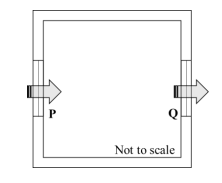
\includegraphics[width=0.5\textwidth]{figures/Q46}
\end{center}
\vspace{0.5cm}

\questionb{A 5m × 5m × 3m room has four 230 mm thick external brick walls. Total wall fenestration is 10 sqm. The temperature difference between indoor and outdoor is 2°C. The air to air transmittance values for 230 mm thick brick wall and 200 mm thick aerated concrete block wall are 2.4 and 1.7 W/sqm°C respectively. If the brick walls are replaced with the aerated concrete block walls, then the change in conductive heat flow through the walls is \_\_\_\_\_ W.}{47}
\vspace{0.5cm}

\questionb{For an activity, 'optimistic time duration' is 4 days, 'pessimistic time duration' is 11 days and 'most-likely time duration' is 8 days. The PERT value of time duration is \_\_\_\_\_ days (up to one decimal place).}{48}
\vspace{0.5cm}

\questionb{In the Figure, the negative bending moment at point A of the cantilever is \_\_\_\_\_ kNm.}{49}
\begin{center}
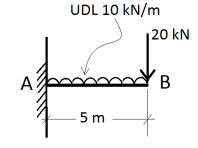
\includegraphics[width=0.5\textwidth]{figures/Q49}
\end{center}
\vspace{0.5cm}

\questionb{The water consumption of a high rise apartment building with 60 dwelling units having an average household size of 5 persons is 135 lped. Assuming 80\% of the total use is met with recycled water supply, the daily domestic demand for the building is \_\_\_\_\_ litres.}{50}
\vspace{0.5cm}

\questionb{In India, for 1.0 cum of M-20 grade concrete, the number of cement bags required is \_\_\_\_\_ (up to two decimal places).}{51}
\vspace{0.5cm}

\questionb{The sound power level of an outdoor non-directional point source is 90 dB. Considering an atmospheric impedance of 400 rayls, the sound pressure level at 10 m distance from the source is \_\_\_\_\_ dB.}{52}
\vspace{0.5cm}

\questionb{The live load and dead load in a three storeyed residential building, transferred through a single column, is 12 tons and 18 tons respectively. If the soil bearing capacity is 10 ton/sqm and the factor of safety is 1.5, the area of column footing is \_\_\_\_\_ sqm (up to one decimal place).}{53}
\vspace{0.5cm}

\questionb{The indoor illumination requirement for a building is 350 Lux. If the daylight factor is 2.7\% and the design sky illuminance is 9000 Lux, then the required supplementary artificial lighting is \_\_\_\_\_ Lux.}{54}
\vspace{0.5cm}

\questionb{Two design options of a business building on a 10.0 hectare site are being compared for built up area. Floor to floor height of Option A is 3.6 m and that of Option B is 4.5 m. If the maximum allowable building height is 45 m with same ground coverage for both options, the additional built up area achievable in Option A over Option B is \_\_\_\_\_ percent.}{55}
\vspace{1cm}

\begin{center}
\textbf{END OF THE QUESTION PAPER}
\rule{\textwidth}{0.5pt} 
\end{center}

\end{document}